\documentclass[tikz,border=5]{standalone}
\usetikzlibrary{decorations.pathmorphing}
\usepackage[detect-all]{siunitx}

\tikzset{
   ragged border/.style={ decoration={random steps, segment length=1mm, amplitude=0.5mm},
           decorate,
   }
}

\def\pp{0001}

\begin{document}
  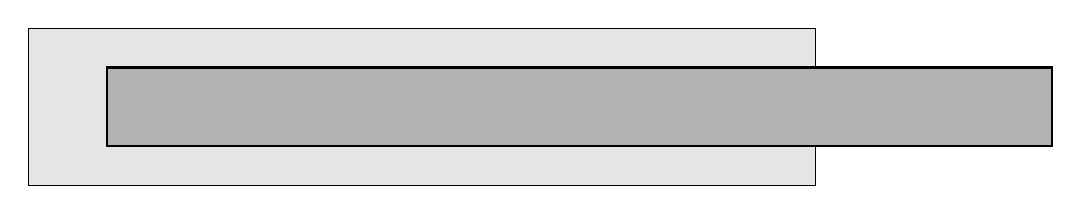
\begin{tikzpicture}
    \draw[fill=black!10] (0,-1) rectangle (10,1);
    \draw[thick, fill=black!30] (\pp, -0.5) rectangle ++(12, 1);
  \end{tikzpicture}
\end{document}